\documentclass[12pt, answers]{exam}

\title{Revision Practice}
\author{T2W10 HBL}
\date{26 May 2022}

\usepackage{amsmath, siunitx}
\usepackage{notomath, noto-mono}

\usepackage{tikz, pgfplots}
\pgfplotsset{compat=1.9}
\usepgfplotslibrary{external}
\tikzexternalize

\usepackage{graphicx}

\renewcommand{\half}{\dfrac{1}{2}}
\newcommand{\Half}{\frac{1}{2}}
\newcommand{\third}{\dfrac{1}{3}}
\newcommand{\oneover}[1]{\dfrac{1}{#1}}
\newcommand{\kg}{\kilo\gram}
\newcommand{\cm}{\centi\metre}

\begin{document}
\maketitle

\begin{questions}
\question The diagram shows a quadratic curve which can be expressed in the form of $y = ax^2 + bx + c$.
Given that the curve cuts the $x$-axis at $2$ and $8$ and the $y$-axis at $-8$,
find the values of $a$, $b$ and $c$.

\begin{figure}[htpb]
    \centering
    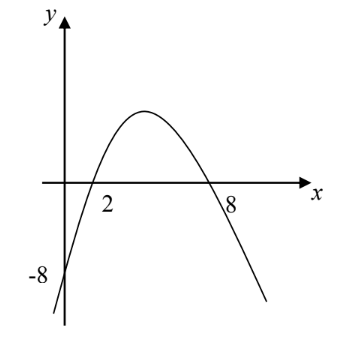
\includegraphics{graphq1.png}
    \label{fig:q1}
\end{figure}

\begin{solution}
\begin{align*}
    0 &= a(x - 2)(x - 8) \\
    y &= a(x - 2)(x - 8) \\
\end{align*}
Using the fact that the graph intercepts $(0, -8)$,
\begin{align*}
    -8 &= a(0 - 2)(0 - 8) \\
    16a &= -8 \\
    a &= -\half \\
    \therefore y &= -\half(x - 2)(x - 8) \\
    &= -\half x^2 + 5x - 8 \\
    \therefore a = -\half,\; b &= 5,\; c = -8
\end{align*}
\end{solution}

\question In the diagram, $\angle ABC = $ \ang{90},
$AC = $ \qty{41}{\cm}. $D$ is on $AB$ such that $CD = $ \qty{15}{\cm}, $BD = $ \qty{12}{\cm}.
Calculate the value of $BC$ and of $AD$.

\begin{figure}[htpb]
    \centering
    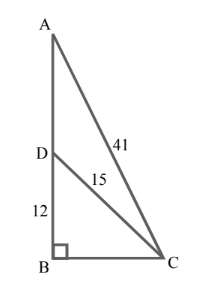
\includegraphics{triq2.png}
    \label{fig:q2}
\end{figure}

\begin{solution}
\begin{align*}
    BC &= \sqrt{15^2 - 12^2} \\
    &= \qty{9}{\cm} \\
    AD &= \sqrt{41^2 - BC^2} - BD \\
    &= \sqrt{41^2 - 9^2} - 12 \\
    &= \qty{28}{\cm} 
\end{align*}
\end{solution}

\question Solve for $x$ in the following equations.

\begin{parts}
\part ${2006}^{x^2 - 9x + 20} - 1 = 0$
\begin{solution}
\begin{align*}
    {2006}^{x^2 - 9x + 20} - 1 &= 0 \\
    x^2 - 9x + 20 &= 0 \\
    (x - 4)(x - 5) &= 0 \\
    x &= 4 \text{ or } 5
\end{align*}
\end{solution}

\part $4^x \left( 5^{2x} \right) = 10$
\begin{solution}
\begin{align*}
    4^x \left( 5^{2x} \right) &= 10 \\
    4^x \cdot {\left( 5^2 \right)}^x &= 10 \\
    4^x \cdot {25}^x &= 10 \\
    {100}^x &= 10 \\
    {\left( {10}^2 \right)}^x &= {10}^1 \\
    2x &= 1 \\
    x &= \half
\end{align*}
\end{solution}

\part $3^{14} \left( 9^{1 - x} \right) = {\left( 3^3 \right)}^{2x}$
\begin{solution}
\begin{align*}
    3^{14} \left( 9^{1 - x} \right) &= {\left( 3^3 \right)}^{2x} \\
    3^{14} \cdot 3^{2 - 2x} &= 3^{6x} \\
    16 - 2x &= 6x \\
    x &= 2
\end{align*}
\end{solution}

\part ${25}^{x + 2} = {125}^{4 - x}$
\begin{solution}
\begin{align*}
    {25}^{x + 2} &= {125}^{4 - x} \\
    5^{2x + 4} &= 5^{12 - 3x} \\
    2x + 4 &= 12 - 3x \\
    x &= \dfrac{8}{5}
\end{align*}
\end{solution}

\part $\sqrt{m\sqrt{m\sqrt{m}}} = m^{x - 1}$
\begin{solution}
\begin{align*}
    \sqrt{m\sqrt{m\sqrt{m}}} &= m^{x - 1} \\
    \sqrt{m\sqrt{m^{\frac{3}{2}}}} &= m^{x - 1} \\
    \sqrt{m^{\frac{7}{4}}} &= m^{x - 1} \\
    m^{\frac{7}{8}} &= m^{x - 1} \\
    x - 1 &= \dfrac{7}{8} \\
    x &= \dfrac{15}{8}
\end{align*}
\end{solution}
\end{parts}

\question It is given that Newton's Law of Universal Gravitation is defined by the formula $F = \dfrac{GMm}{r^2}$.

\begin{parts}
\part Make $r$ the subject of the formula.
\begin{solution}
\begin{align*}
    F &= \dfrac{GMm}{r^2} \\
    r^2 &= \dfrac{GMm}{F} \\
    r &= \pm \sqrt{\dfrac{GMm}{F}}
\end{align*}
\end{solution}

\part Find the positive value of $r$ (correct to the nearest whole number) if $G = $ \num{6.67e-11}, $M = $ \num{6.6e21}, $m = $ \num{1.5e2} and $F = 1.43$.

\begin{solution}
\begin{align*}
    r &= \sqrt{\dfrac{GMm}{F}} \\
    &= \sqrt{\dfrac{\num{6.67e-11} \times \num{6.6e21} \times \num{1.5e2}}{1.43}} \\
    &= \sqrt{\dfrac{\num{66.033e12}}{1.43}} \\
    &=\num{6795360} \text{ (nearest whole number)}
\end{align*}
\end{solution}
\end{parts}

\question Simplify the following expressions.
\begin{parts}
\part ${\left(a^2b^{-3}\right)}^3 \times \dfrac{ab^{-2}}{a^3}$
\begin{solution}
\begin{align*}
    {\left(a^2b^{-3}\right)}^3 \times \dfrac{ab^{-2}}{a^3} &= \dfrac{a^6b^{-9} \times ab^{-2}}{a^3} \\
    &= \dfrac{a^7}{a^3b^{11}} \\
    &= \dfrac{a^4}{b^{11}}
\end{align*}
\end{solution}

\part $\left(a^3b\right)^{-2} \div \left(a^2b^{-5}\right) \times \dfrac{a^3}{b^7}$
\begin{solution}
\begin{align*}
    \left(a^3b\right)^{-2} \div \left(a^2b^{-5}\right) \times \dfrac{a^3}{b^7} &= \dfrac{a^{-6}b^{-2}}{a^2b^{-5}} \times \dfrac{a^3}{b^7} \\
    &= \dfrac{b^3}{a^8} \times \dfrac{a^3}{b^7} \\
    &= \oneover{a^5b^4}
\end{align*}
\end{solution}

\part $\left(3a^{-2}b^2\right)^3 \times \left(6a^3b^{-2}\right)^{-2}$
\begin{solution}
\begin{align*}
    \left(3a^{-2}b^2\right)^3 \times \left(6a^3b^{-2}\right)^{-2} &= 27a^{-6}b^6 \times \oneover{36} a^{-6}b^4 \\
    &= \dfrac{27a^{-12}b^{10}}{36} \\
    &= \dfrac{3b^{10}}{4a^{12}}
\end{align*}
\end{solution}

\part $\left(5a^{-4}b^5\right)^{-1} \times 6\left(a^2b\right)^{-3}$
\begin{solution}
\begin{align*}
    \left(5a^{-4}b^5\right)^{-1} \times 6\left(a^2b\right)^{-3} &= \dfrac{a^4}{5b^5} \times \dfrac{6}{a^6b^3} \\
    &= \dfrac{6}{5a^2b^8}
\end{align*}
\end{solution}

\part $\dfrac{7m^{\frac{5}{3}}n^3}{2p} \div \dfrac{21m^{\frac{2}{3}}n^4}{6p^2}$
\begin{solution}
\begin{align*}
    \dfrac{7m^{\frac{5}{3}}n^3}{2p} \div \dfrac{21m^{\frac{2}{3}}n^4}{6p^2} &= \dfrac{7m^{\frac{5}{3}}n^3}{2p} \times \dfrac{6p^2}{21m^{\frac{2}{3}}n^4} \\
    &= m \times \dfrac{3p}{3n} \\
    &= \dfrac{mp}{n}
\end{align*}
\end{solution}

\part $4^x \times 8^{x + 2} \times 6^{2x - 2}$
\begin{solution}
\begin{align*}
    4^x \times 8^{x + 2} \times 6^{2x - 2} &= 2^{2x + 3x + 6} \times 2^{2x - 2} \times 3^{2x - 2} \\
    &= 2^{7x + 4} \times 3^{2x - 2}
\end{align*}
\end{solution}

\part $\dfrac{\sqrt{x^{-2}y^4}}{\left(\dfrac{x}{y}\right)^{-2}}$
\begin{solution}
\begin{align*}
    \dfrac{\sqrt{x^{-2}y^4}}{\left(\dfrac{x}{y}\right)^{-2}} &= \dfrac{x^{-1}y^2}{\dfrac{y^2}{x^2}} \\
    &= \dfrac{xy^2}{y^2} \\
    &= x
\end{align*}
\end{solution}

\part $\dfrac{\left(2p^4q^3\right)^3}{4p^2q^{15}}$
\begin{solution}
\begin{align*}
    \dfrac{\left(2p^4q^3\right)^3}{4p^2q^{15}} &= \dfrac{2p^{12}q^9}{p^2q^{15}} \\
    &= \dfrac{2p^{10}}{q^6}
\end{align*}
\end{solution}
\end{parts}

\question The figure below shows a right-angled triangle with sides $x$ \si{\cm}, \qty{5}{\cm} and $(x + 1)$ \si{\cm} respectively.
Write down an equation in $x$, and, hence, find the value of $x$.
\begin{figure}[htpb]
    \centering
    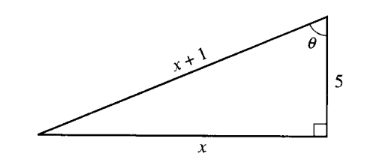
\includegraphics{triq6.png}
    \label{fig:q6}
\end{figure}
\begin{solution}
\begin{align*}
    5^2 + x^2 &= \left(x + 1\right)^2 \\
    x^2 + 25 &= x^2 + 2x + 1 \\
    2x &= 24 \\
    x &= 12
\end{align*}
\end{solution}

\question Evaluate $\dfrac{\num{9.016e3} + \num{6.292e4}}{\num{5.673e-2} - \sqrt{\num{2.490e-5}}}$ using a calculator,
leaving your answer in standard form, correct to three significant figures.
\begin{solution}
\begin{align*}
    \dfrac{\num{9.016e3} + \num{6.292e4}}{\num{5.673e-2} - \sqrt{\num{2.490e-5}}} &\approx \num{1390336.028} \\
    &\approx \num{1.39e6} \text{ (3 s.f.)}
\end{align*}
\end{solution}

\question The diagonal of the square base of the right pyramid below is \qty{18}{\cm} and the slant edge, $VC$ is \qty{15}{\cm}.
Calculate
\begin{figure}[htpb]
    \centering
    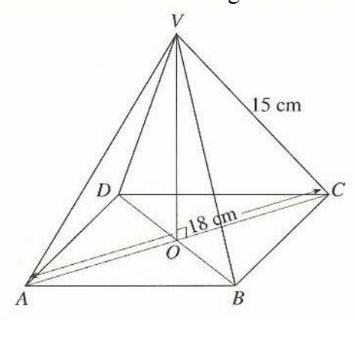
\includegraphics{pyrq8.png}
    \label{fig:q8}
\end{figure}

\begin{parts}
\part the height of the pyramid,
\begin{solution}
\begin{align*}
    \text{height of pyramid } &= \sqrt{15^2 - \left(\dfrac{18}{2}\right)^2} \\
    &= \qty{12}{\cm}
\end{align*}
\end{solution}
\part the volume of the pyramid.
\begin{solution}
\begin{align*}
    \text{volume of pyramid } &= \third \times \left(2 \times \half \times 18 \times \dfrac{18}{2}\right) \times 12 \\
    &= \qty{648}{\cubic\cm}
\end{align*}
\end{solution}
\end{parts}

\question The diagram below shows a semicircle with $O$ as centre and $AB$ as diameter.
$C$ is a point on the circumference such that $BC = $ \qty{7}{\cm} and
$AC = (2a - 3b)$ \si{\cm}. Given that $OA = $ \qty{12.5}{\cm} and $OB = (a - 2b)$ \si{\cm},
\begin{figure}[htpb]
    \centering
    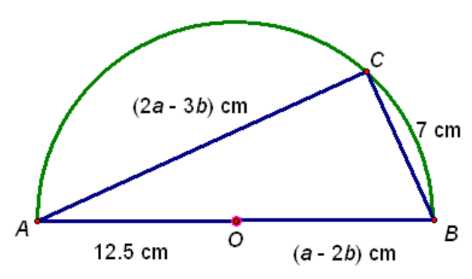
\includegraphics{semiq9.png}
    \label{fig:q9}
\end{figure}

\begin{parts}
\part \label{9a} By considering the diameter of the circle, write down an equation involving $a$ and $b$.
\begin{solution}
$a - 2b = 12.5$
\end{solution}

\part \label{9b} By using the Pythagoras Theorem, form another equation involving $a$ and $b$.
\begin{solution}
\begin{align*}
    7^2 + (2a - 3b)^2 &= \left[2(a - 2b)\right]^2 \\
    49 + 4a^2 - 12ab + 9b^2 &= (2a - 4b)^2 \\
    4a^2 - 12ab + 9b^2 + 49 &= 4a^2 - 16ab + 16b^2 \\
    4ab + 49 &= 7b^2
\end{align*}
\end{solution}

\part Find the values of $a$ and $b$ by solving the equations obtained in \textbf{(\ref{9a})} and \textbf{(\ref{9b})} simultaneously.
\begin{solution}
\begin{align*}
    a - 2b &= 12.5\label{eq:91}\tag{1} \\
    4ab + 49 &= 7b^2\label{eq:92}\tag{2}
\end{align*}
From \eqref{eq:92}:
\begin{align*}
    4ab + 49 &= 7b^2 \\
4ab &= 7b^2 - 49 \\
a &= \dfrac{7b^2 - 49}{4b}\label{eq:93}\tag{3}
\end{align*}
Substitute \eqref{eq:93} into \eqref{eq:91}:
\begin{align*}
    \dfrac{7b^2 - 49}{4b} - 2b &= 12.5 \\
    7b^2 - 49 - 8b^2 &= 50b \\
    b^2 + 50b + 49 &= 0
    (b + 49)(b + 1) &= 0 \\
    \therefore b &= -1 \text{ or } b = -49
\end{align*}
Substitute $b = -1$ into \eqref{eq:91}:
\begin{align*}
    a + 2 &= 12.5 \\
    \therefore a &= 10.5
\end{align*}
Substitute $b = -49$ into \eqref{eq:91}:
\begin{align*}
    a + 98 &= 12.5 \\
    \therefore a &= -85.5 \text{ (rej.)}
\end{align*}
\[
\therefore \begin{cases}
a &= 10.5 \\
b &= -1 
\end{cases}
\]
\end{solution}
\end{parts}

\question Evaulate
\begin{parts}
\part ${27}^{\frac{3}{5}} \div {27}^{\frac{2}{5}} \times {27}^{\frac{2}{15}}$
\begin{solution}
\begin{align*}
    {27}^{\frac{3}{5}} \div {27}^{\frac{2}{5}} \times {27}^{\frac{2}{15}} &= {27}^{\frac{3}{5} - \frac{2}{5} + \frac{1}{15}} \\
    &= {27}^{\frac{4}{15}}
\end{align*}
\end{solution}
\part $\left(-2\right)^{-3}$
\begin{solution}
\begin{align*}
    \left(-2\right)^{-3} &= \oneover{\left(-2\right)^3} \\
    &= -\oneover{8}
\end{align*}
\end{solution}

\part $\left(\dfrac{343}{64}\right)^{-\frac{2}{3}}$ 
\begin{solution}
\begin{align*}
    \left(\dfrac{343}{64}\right)^{-\frac{2}{3}} &= \left(\dfrac{64}{343}\right)^{\frac{2}{3}} \\
    &= \sqrt[3]{\left(\dfrac{64}{343}\right)^2} \\
    &= \sqrt[3]{\dfrac{2^{12}}{7^6}} \\
    &= \dfrac{2^4}{7^2} \\
    &= \dfrac{16}{49}
\end{align*}
\end{solution}

\part $\left(\half\right)^{-2} \times 2^0$
\begin{solution}
\begin{align*}
    \left(\half\right)^{-2} \times 2^0 &= 2^2 \\
    &= 4
\end{align*}
\end{solution}
\end{parts}

\question For the given figure, find

\begin{figure}[htpb]
    \centering
    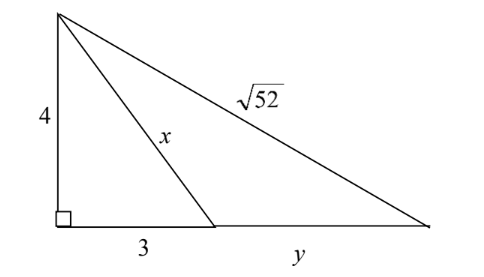
\includegraphics{triq11.png}
    \label{fig:q11}
\end{figure}

\begin{parts}
\part $x$,
\begin{solution}
\begin{align*}
x &= \sqrt{3^2 + 4^2} \\
&= 5
\end{align*}
\end{solution}
\part $y$.
\begin{solution}
\begin{align*}
    y &= \sqrt{\left(\sqrt{52}\right)^2 - 4^2} - 3 \\
    &= 3
\end{align*}
\end{solution}
\end{parts}

\question A circle, centre $O$, radius $x$ \si{\cm}, has a chord $AB$ of length $20\sqrt{2}$ \si{\cm}.
$\angle AOB = $ \ang{90}.
Find 
\begin{figure}[htpb]
    \centering
    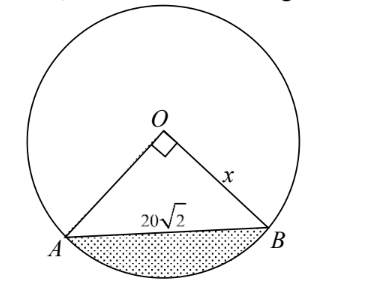
\includegraphics{circq12.png}
    \label{fig:q12}
\end{figure}

\begin{parts}
\part the value of $x$,
\begin{solution}
\begin{align*}
    x &= \sqrt{\dfrac{\left(20\sqrt{2}\right)^2}{2}}\\
    &= 20
\end{align*}
\end{solution}

\part the area of the shaded region correct to the nearest \qty{5}{\square\cm}.
\begin{solution}
\begin{align*}
\text{area of the shaded region } &= \oneover{4} \times \pi \times {20}^2 - \half \times {20^2} \\
&= \qty{114}{\square\cm} \\
&= \qty{115}{\square\cm} \text{ (nearest \qty{5}{\square\cm})}
\end{align*}
\end{solution}
\end{parts}
\end{questions}
\end{document}
